\documentclass[14pt]{extbook}
\usepackage{multicol, enumerate, enumitem, hyperref, color, soul, setspace, parskip, fancyhdr} %General Packages
\usepackage{amssymb, amsthm, amsmath, bbm, latexsym, units, mathtools} %Math Packages
\everymath{\displaystyle} %All math in Display Style
% Packages with additional options
\usepackage[headsep=0.5cm,headheight=12pt, left=1 in,right= 1 in,top= 1 in,bottom= 1 in]{geometry}
\usepackage[usenames,dvipsnames]{xcolor}
\usepackage{dashrule}  % Package to use the command below to create lines between items
\newcommand{\litem}[1]{\item#1\hspace*{-1cm}\rule{\textwidth}{0.4pt}}
\pagestyle{fancy}
\lhead{Makeup Progress Quiz 3}
\chead{}
\rhead{Version A}
\lfoot{4315-3397}
\cfoot{}
\rfoot{Fall 2020}
\begin{document}

\begin{enumerate}
\litem{
Construct the lowest-degree polynomial given the zeros below. Then, choose the intervals that contain the coefficients of the polynomial in the form $ax^3+bx^2+cx+d$.\[ \frac{-4}{5}, 2, \text{ and } \frac{7}{5} \]\begin{enumerate}[label=\Alph*.]
\item \( a \in [24, 31], b \in [-72, -62], c \in [1, 7], \text{ and } d \in [-56, -55] \)
\item \( a \in [24, 31], b \in [57, 69], c \in [1, 7], \text{ and } d \in [-56, -55] \)
\item \( a \in [24, 31], b \in [-72, -62], c \in [1, 7], \text{ and } d \in [53, 61] \)
\item \( a \in [24, 31], b \in [-105, -101], c \in [138, 141], \text{ and } d \in [-56, -55] \)
\item \( a \in [24, 31], b \in [-11, -3], c \in [-87, -79], \text{ and } d \in [53, 61] \)

\end{enumerate} }
\litem{
Construct the lowest-degree polynomial given the zeros below. Then, choose the intervals that contain the coefficients of the polynomial in the form $x^3+bx^2+cx+d$.\[ 2 + 4 i \text{ and } -4 \]\begin{enumerate}[label=\Alph*.]
\item \( b \in [-1.82, 0.38], c \in [3.17, 4.11], \text{ and } d \in [79, 85] \)
\item \( b \in [-1.82, 0.38], c \in [3.17, 4.11], \text{ and } d \in [-80, -76] \)
\item \( b \in [0.07, 1.76], c \in [1.42, 3.02], \text{ and } d \in [-10, -5] \)
\item \( b \in [0.07, 1.76], c \in [-0.67, 0.1], \text{ and } d \in [-18, -10] \)
\item \( \text{None of the above.} \)

\end{enumerate} }
\litem{
Construct the lowest-degree polynomial given the zeros below. Then, choose the intervals that contain the coefficients of the polynomial in the form $x^3+bx^2+cx+d$.\[ 3 + 4 i \text{ and } 2 \]\begin{enumerate}[label=\Alph*.]
\item \( b \in [0, 2], c \in [-6.65, -5.66], \text{ and } d \in [8, 12] \)
\item \( b \in [-14, -4], c \in [37, 37.08], \text{ and } d \in [-56, -49] \)
\item \( b \in [6, 11], c \in [37, 37.08], \text{ and } d \in [47, 56] \)
\item \( b \in [0, 2], c \in [-5.69, -4.9], \text{ and } d \in [3, 7] \)
\item \( \text{None of the above.} \)

\end{enumerate} }
\litem{
Construct the lowest-degree polynomial given the zeros below. Then, choose the intervals that contain the coefficients of the polynomial in the form $ax^3+bx^2+cx+d$.\[ -6, \frac{-7}{4}, \text{ and } \frac{1}{4} \]\begin{enumerate}[label=\Alph*.]
\item \( a \in [11, 21], b \in [117, 121], c \in [134, 138], \text{ and } d \in [-47, -41] \)
\item \( a \in [11, 21], b \in [-122, -115], c \in [134, 138], \text{ and } d \in [42, 43] \)
\item \( a \in [11, 21], b \in [-72, -70], c \in [-152, -143], \text{ and } d \in [42, 43] \)
\item \( a \in [11, 21], b \in [117, 121], c \in [134, 138], \text{ and } d \in [42, 43] \)
\item \( a \in [11, 21], b \in [-131, -122], c \in [197, 201], \text{ and } d \in [-47, -41] \)

\end{enumerate} }
\litem{
Describe the zero behavior of the zero $x = -7$ of the polynomial below.\[ f(x) = 9(x + 7)^{8}(x - 7)^{9}(x + 3)^{4}(x - 3)^{5} \]\begin{enumerate}[label=\Alph*.]
\begin{multicols}{2}\item 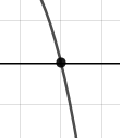
\includegraphics[width = 0.3\textwidth]{../Figures/polyZeroBehaviorAA.png}\item 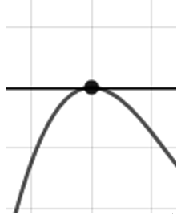
\includegraphics[width = 0.3\textwidth]{../Figures/polyZeroBehaviorBA.png}\item 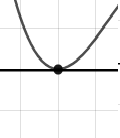
\includegraphics[width = 0.3\textwidth]{../Figures/polyZeroBehaviorCA.png}\item 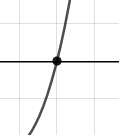
\includegraphics[width = 0.3\textwidth]{../Figures/polyZeroBehaviorDA.png}\end{multicols}\item None of the above.
\end{enumerate} }
\litem{
Which of the following equations \textit{could} be of the graph presented below?
\begin{center}
    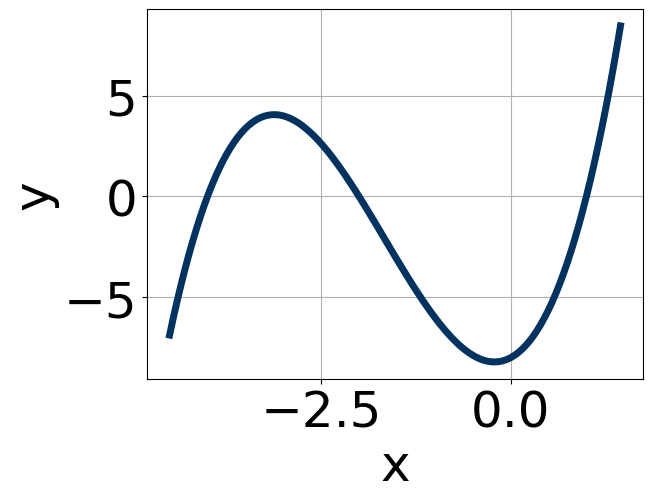
\includegraphics[width=0.5\textwidth]{../Figures/polyGraphToFunctionCopyA.png}
\end{center}
\begin{enumerate}[label=\Alph*.]
\item \( 12(x + 4)^{10} (x - 1)^{11} (x + 2)^{5} \)
\item \( 14(x + 4)^{10} (x - 1)^{6} (x + 2)^{11} \)
\item \( -6(x + 4)^{6} (x - 1)^{5} (x + 2)^{9} \)
\item \( -9(x + 4)^{9} (x - 1)^{7} (x + 2)^{5} \)
\item \( 12(x + 4)^{7} (x - 1)^{7} (x + 2)^{5} \)

\end{enumerate} }
\litem{
Describe the zero behavior of the zero $x = 7$ of the polynomial below.\[ f(x) = -4(x + 2)^{5}(x - 2)^{3}(x + 7)^{7}(x - 7)^{6} \]\begin{enumerate}[label=\Alph*.]
\begin{multicols}{2}\item 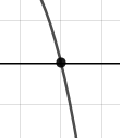
\includegraphics[width = 0.3\textwidth]{../Figures/polyZeroBehaviorCopyAA.png}\item 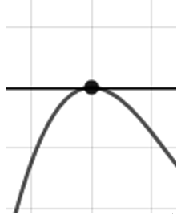
\includegraphics[width = 0.3\textwidth]{../Figures/polyZeroBehaviorCopyBA.png}\item 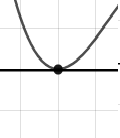
\includegraphics[width = 0.3\textwidth]{../Figures/polyZeroBehaviorCopyCA.png}\item 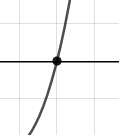
\includegraphics[width = 0.3\textwidth]{../Figures/polyZeroBehaviorCopyDA.png}\end{multicols}\item None of the above.
\end{enumerate} }
\litem{
Which of the following equations \textit{could} be of the graph presented below?
\begin{center}
    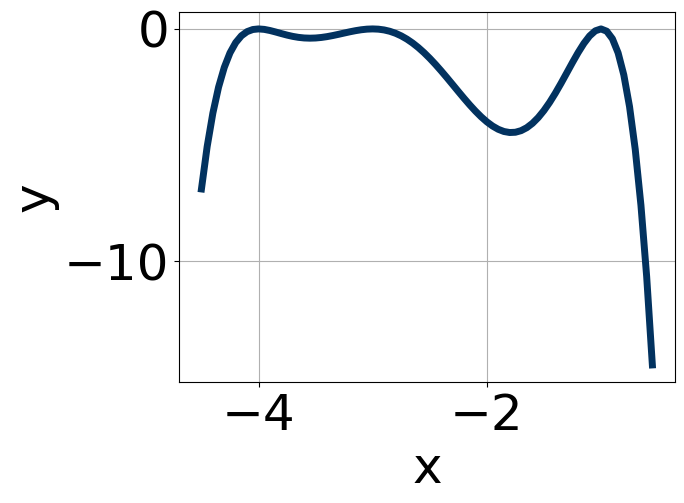
\includegraphics[width=0.5\textwidth]{../Figures/polyGraphToFunctionA.png}
\end{center}
\begin{enumerate}[label=\Alph*.]
\item \( 10(x + 3)^{10} (x + 4)^{8} (x + 1)^{10} \)
\item \( -12(x + 3)^{10} (x + 4)^{6} (x + 1)^{4} \)
\item \( 7(x + 3)^{8} (x + 4)^{8} (x + 1)^{11} \)
\item \( -6(x + 3)^{4} (x + 4)^{11} (x + 1)^{9} \)
\item \( -19(x + 3)^{6} (x + 4)^{8} (x + 1)^{7} \)

\end{enumerate} }
\litem{
Describe the end behavior of the polynomial below.\[ f(x) = -8(x + 2)^{3}(x - 2)^{8}(x - 5)^{5}(x + 5)^{5} \]\begin{enumerate}[label=\Alph*.]
\begin{multicols}{2}\item 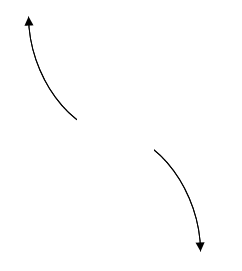
\includegraphics[width = 0.3\textwidth]{../Figures/polyEndBehaviorCopyAA.png}\item 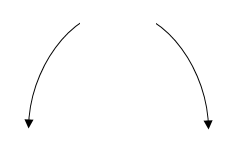
\includegraphics[width = 0.3\textwidth]{../Figures/polyEndBehaviorCopyBA.png}\item 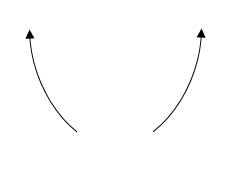
\includegraphics[width = 0.3\textwidth]{../Figures/polyEndBehaviorCopyCA.png}\item 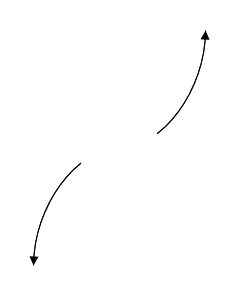
\includegraphics[width = 0.3\textwidth]{../Figures/polyEndBehaviorCopyDA.png}\end{multicols}\item None of the above.
\end{enumerate} }
\litem{
Describe the end behavior of the polynomial below.\[ f(x) = -5(x - 3)^{4}(x + 3)^{7}(x - 5)^{5}(x + 5)^{6} \]\begin{enumerate}[label=\Alph*.]
\begin{multicols}{2}\item 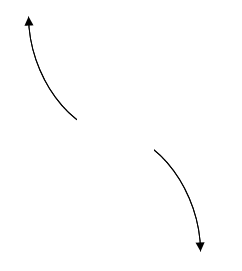
\includegraphics[width = 0.3\textwidth]{../Figures/polyEndBehaviorAA.png}\item 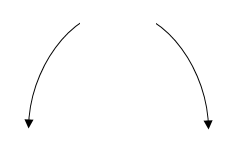
\includegraphics[width = 0.3\textwidth]{../Figures/polyEndBehaviorBA.png}\item 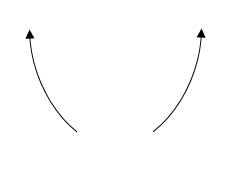
\includegraphics[width = 0.3\textwidth]{../Figures/polyEndBehaviorCA.png}\item 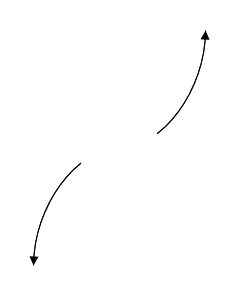
\includegraphics[width = 0.3\textwidth]{../Figures/polyEndBehaviorDA.png}\end{multicols}\item None of the above.
\end{enumerate} }
\end{enumerate}

\end{document}